%%%%%%%%%%%%%%%%%%%%%%%%%%%%%%%%%%%%%%%%%%%%%%%%%%%%%%%%%%%%%%%%%%
%%%%%%%% ICML 2015 EXAMPLE LATEX SUBMISSION FILE %%%%%%%%%%%%%%%%% %%%%%%%%%%%%%%%%%%%%%%%%%%%%%%%%%%%%%%%%%%%%%%%%%%%%%%%%%%%%%%%%%%

% Use the following line _only_ if you're still using LaTeX 2.09.
%\documentstyle[icml2015,epsf,natbib]{article}
% If you rely on Latex2e packages, like most moden people use this:
\documentclass{article}

% use Times
\usepackage{times}
% For figures
\usepackage{graphicx} % more modern
%\usepackage{epsfig} % less modern
\usepackage{subfigure} 

% For citations
\usepackage{natbib}

% For algorithms
\usepackage{algorithm}
\usepackage{algorithmic}

% Packages
%%%%%%%%%%%%%%%%%%%%%%%%%%%%%%%%%%%%%%%%%%%%%%%%%%%%%%%%%%%%%%%%%%%%%%%%%%%%%%%%
\usepackage{calc}
\usepackage{amsmath, amssymb, amsthm} 
\usepackage{parskip}
\usepackage{color,hyperref}
\usepackage{epsfig}
\usepackage{subfigure}
\usepackage{verbatim}
\usepackage{rotating}
% Add my definitions file
\usepackage{kky}
\usepackage{hastieDefns}
\usepackage{multicol}
\usepackage{ifthen}
\usepackage{bbm}
\usepackage{siunitx}
\newenvironment{packed_enum}{
\begin{enumerate}
\setlength{\itemsep}{1pt}
\setlength{\parskip}{0pt}
\setlength{\parsep}{0pt}
}{\end{enumerate}}
%%%%%%%%%%%%%%%%%%%%%%%%%%%%%%%%%%%%%%%%%%%%%%%%%%%%%%%%%%%%%%%%%%%%%%%%%%%%%%%%
% \newcommand{\toworkon}[1]{\textcolor{magenta}{[#1]}}
\newcommand{\toworkon}[1]{}
\newboolean{istwocolumn}
\newboolean{isabridged}
\setboolean{isabridged}{false} % Set to true for abridged version
% \setboolean{isabridged}{true} % Set to true for abridged version



% As of 2011, we use the hyperref package to produce hyperlinks in the
% resulting PDF.  If this breaks your system, please commend out the
% following usepackage line and replace \usepackage{icml2015} with
% \usepackage[nohyperref]{icml2015} above.
\usepackage{hyperref}

% Packages hyperref and algorithmic misbehave sometimes.  We can fix
% this with the following command.
\newcommand{\theHalgorithm}{\arabic{algorithm}}

% Employ the following version of the ``usepackage'' statement for
% submitting the draft version of the paper for review.  This will set
% the note in the first column to ``Under review.  Do not distribute.''
\usepackage{icml2015} 

% Employ this version of the ``usepackage'' statement after the paper has
% been accepted, when creating the final version.  This will set the
% note in the first column to ``Proceedings of the...''
% \usepackage[accepted]{icml2015}


% The \icmltitle you define below is probably too long as a header.
% Therefore, a short form for the running title is supplied here:
\icmltitlerunning{Additive Least Squares Regression}

\begin{document} 
\pdfoutput=1

\twocolumn[
\icmltitle{Penalized Additive Least Squares Models for High Dimensional Nonparametric
Regression and Functional Selection}
% \icmltitle{Additive Gaussian Processes for High Dimensional  
% Optimization and Bandits}

% It is OKAY to include author information, even for blind
% submissions: the style file will automatically remove it for you
% unless you've provided the [accepted] option to the icml2015
% package.

% \icmlauthor{Kirthevasan Kandasamy}{kandasamy@cs.cmu.edu}
% \icmlauthor{Jeff Schneider}{schneide@cs.cmu.edu}
% \icmlauthor{Barnab\'as P\'oczos}{bapoczos@cs.cmu.edu}
% \icmladdress{Carnegie Mellon University, Pittsburgh, PA, USA}

% You may provide any keywords that you 
% find helpful for describing your paper; these are used to populate 
% the "keywords" metadata in the PDF but will not be shown in the document
\icmlkeywords{Kernels, Additive Models }

\vskip 0.3in
]


\newcommand{\insertFigCompToy}{
\begin{figure}
\centering
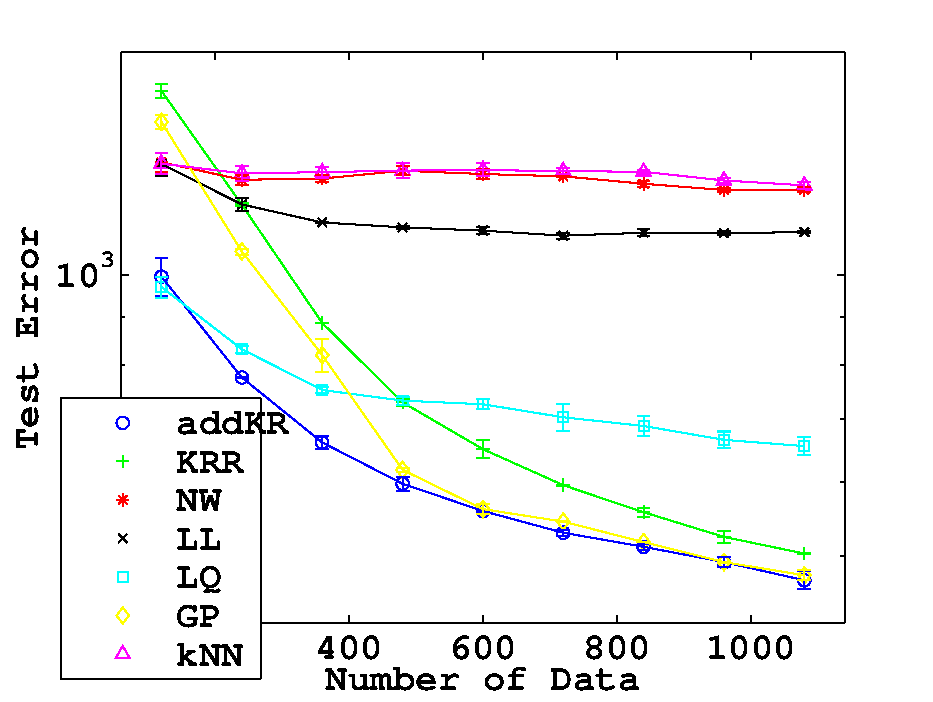
\includegraphics[width=3.2in]{figs/compToy}
\vspace{\imcaptionspace}
\caption[]{\small Comparison of various nonparametric regression methods on a
$20$-dimensional toy dataset. The $x$-axis denotes the number of training data
and the $y$-axis is the test error. }
\vspace{\imtextspace}
\label{fig:compToy}
\end{figure}
}

\newcommand{\insertFigOpt}{
\begin{figure}
\centering
\subfigure[]{
  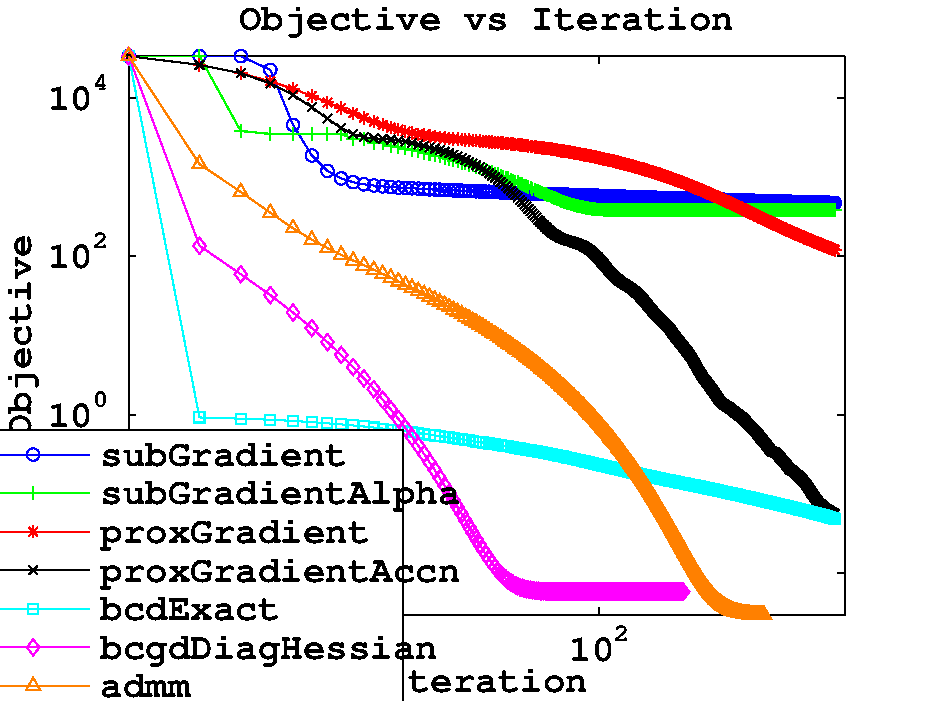
\includegraphics[width=\imarrwtwo]{figs/iteration1000v2} \hspace{\imhsptwo}
  \vspace{\imlabelspace}
  \label{fig:optCompIter}
}
\subfigure[]{
  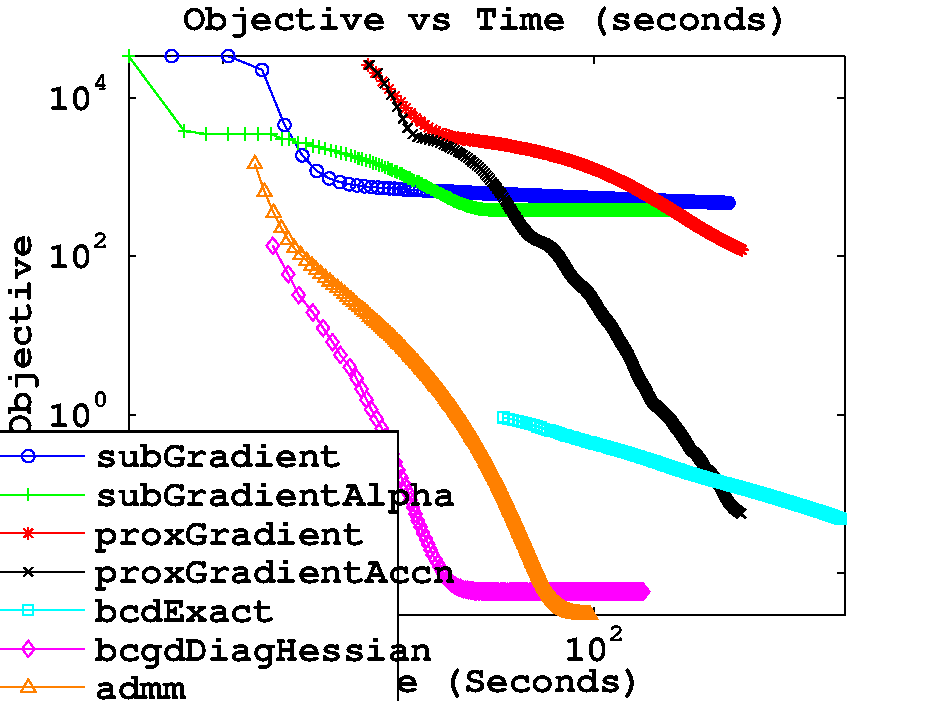
\includegraphics[width=\imarrwtwo]{figs/time1000v2} \hspace{\imhsptwo}
  \vspace{\imlabelspace}
  \label{fig:optCompTime}
}
\caption[]{\small
\subref{fig:optCompIter}: Comparison of the different methods to optimise our
objective. In~\subref{fig:optCompIter} The $x$-axis is the iteration and
in~\subref{fig:optCompTime} the $x$-axis is time. In both figures
 the $y$-axis is the objective. 
Both figures are in log-log scale.
}
\end{figure}
}

\newcommand{\insertFigRegFSel}{
\begin{figure}
\centering
\subfigure[]{
  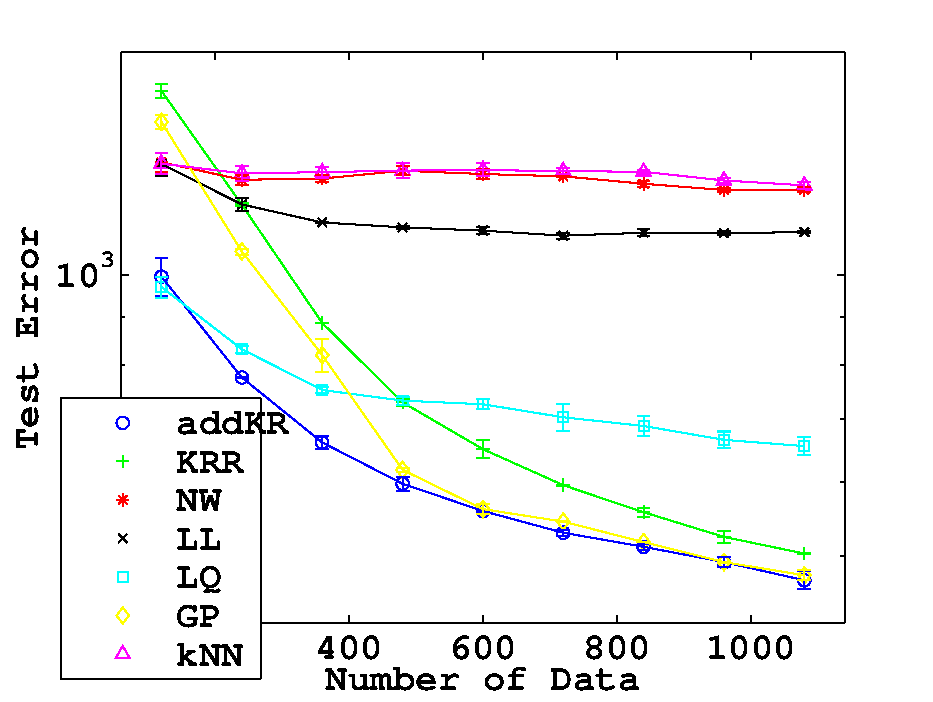
\includegraphics[width=\imarrwtwo]{figs/compToy} \hspace{\imhsptwo}
  \vspace{\imlabelspace}
  \label{fig:compToy}
}
\subfigure[]{
  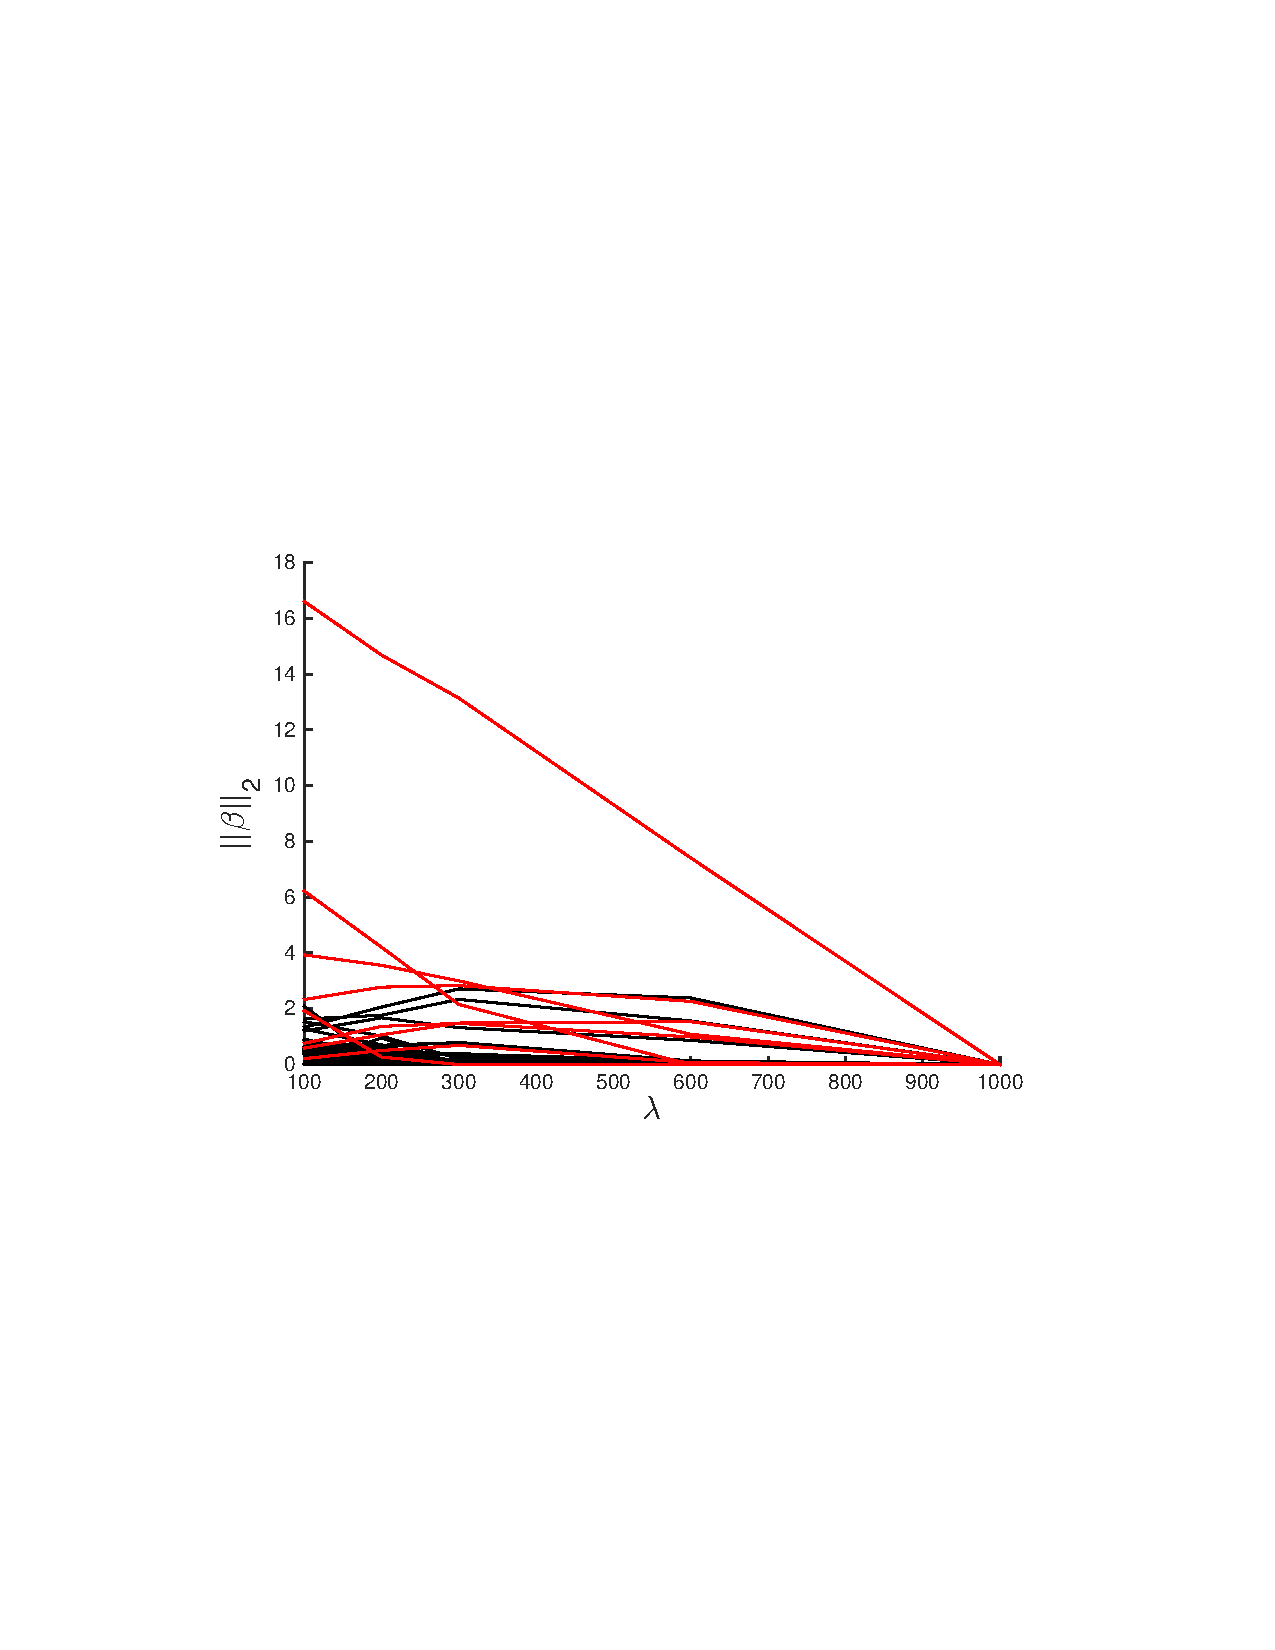
\includegraphics[width=\imarrwtwo]{figs/solnpath600} \hspace{\imhsptwo}
  \vspace{\imlabelspace}
  \label{fig:solnpath}
}
\caption[]{\small
\subref{fig:compToy}: Comparison of \addkrrs using ESP Kernels against other 
nonparametric methods
on a $20$ dimensional toy problem. The $x$-axis denotes the number of training
points and the $y$-axis is the error on a test set.
\subref{fig:solnpath}: Solution path with $n=600$ samples for the synthetic
problem. The $x$-axis shows the regularisation parameter while the $y$-axis
plots $\|\funcj\|_{\Hcalkj} = \|\betaj\|$. The true nonzero functions are
depicted in red. As the figure indicates several of the false functions are
driven to $0$ fast whereas the true functions persist for longer.
}
\end{figure}
}



\newcommand{\insertFigSolnPath}{
\begin{figure}
\centering
% 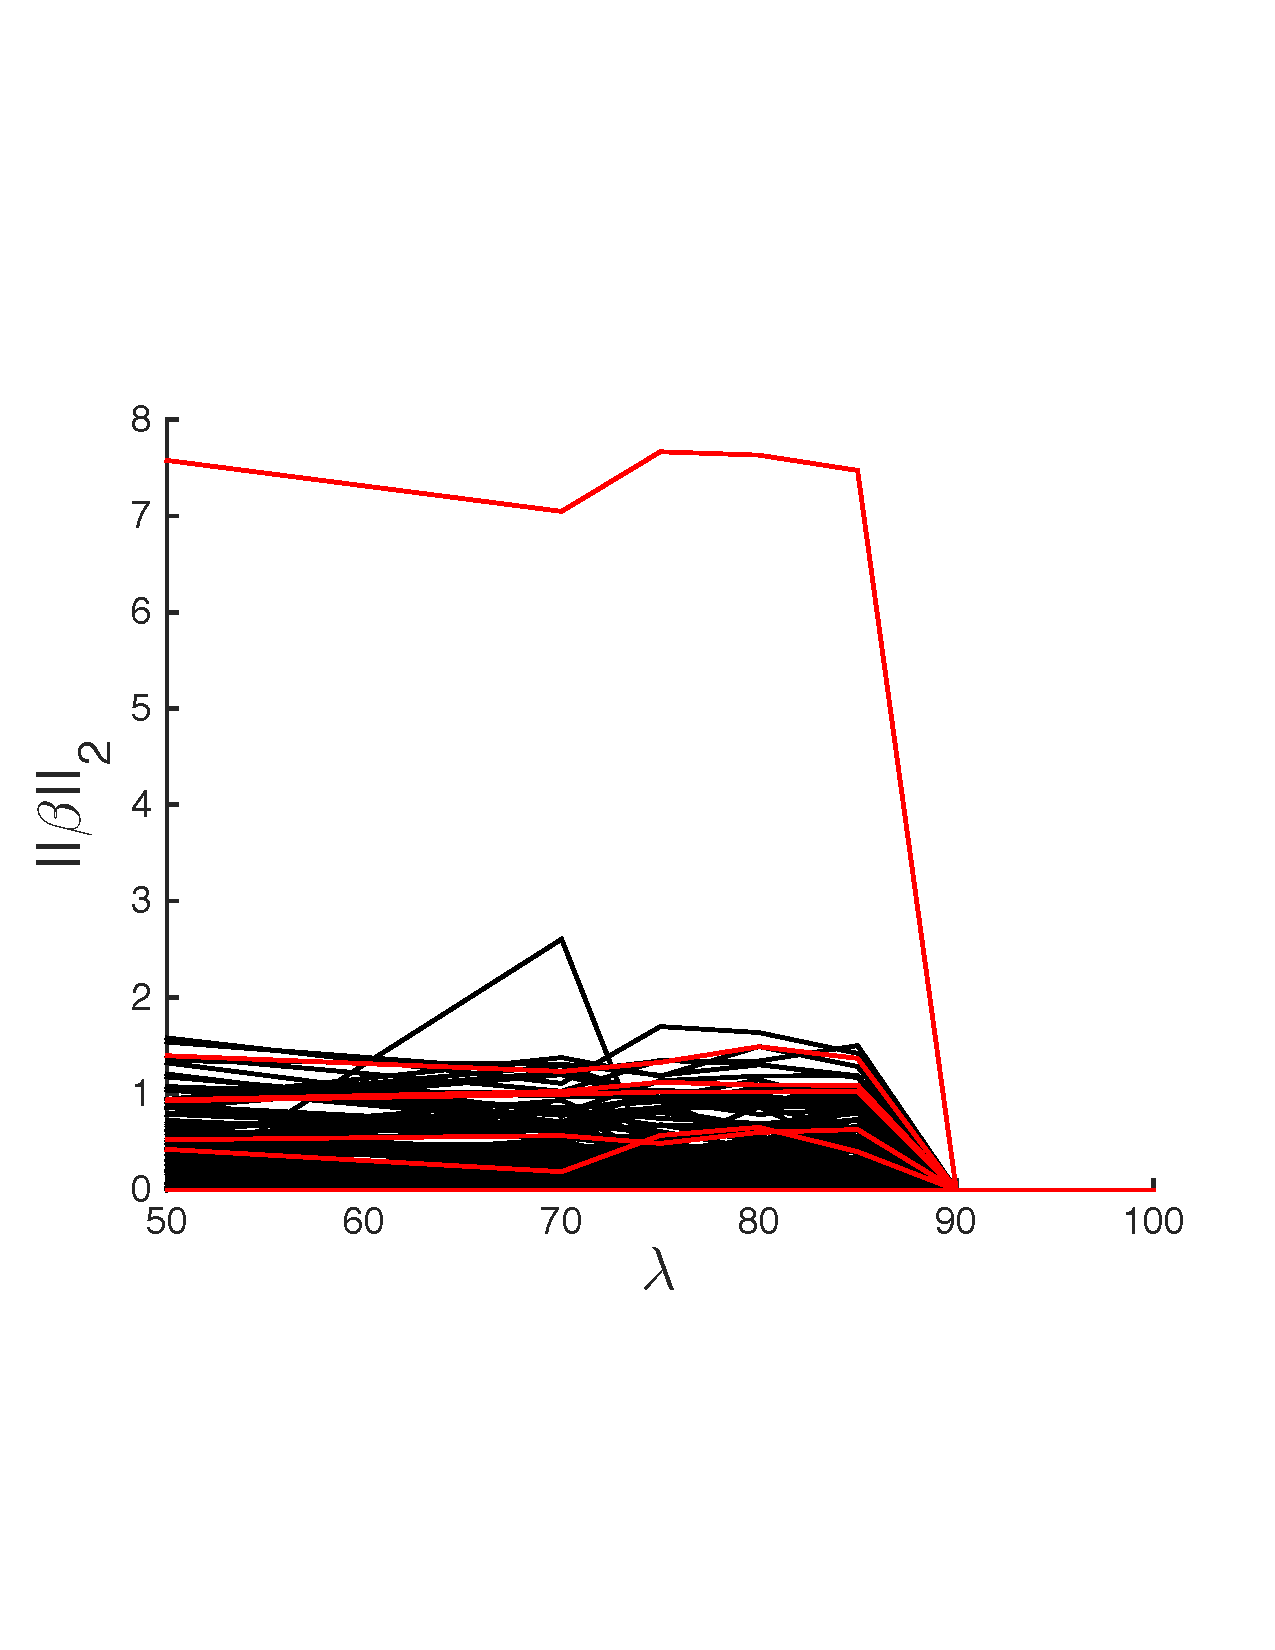
\includegraphics[width=3.4in]{figs/solnpath200.pdf}
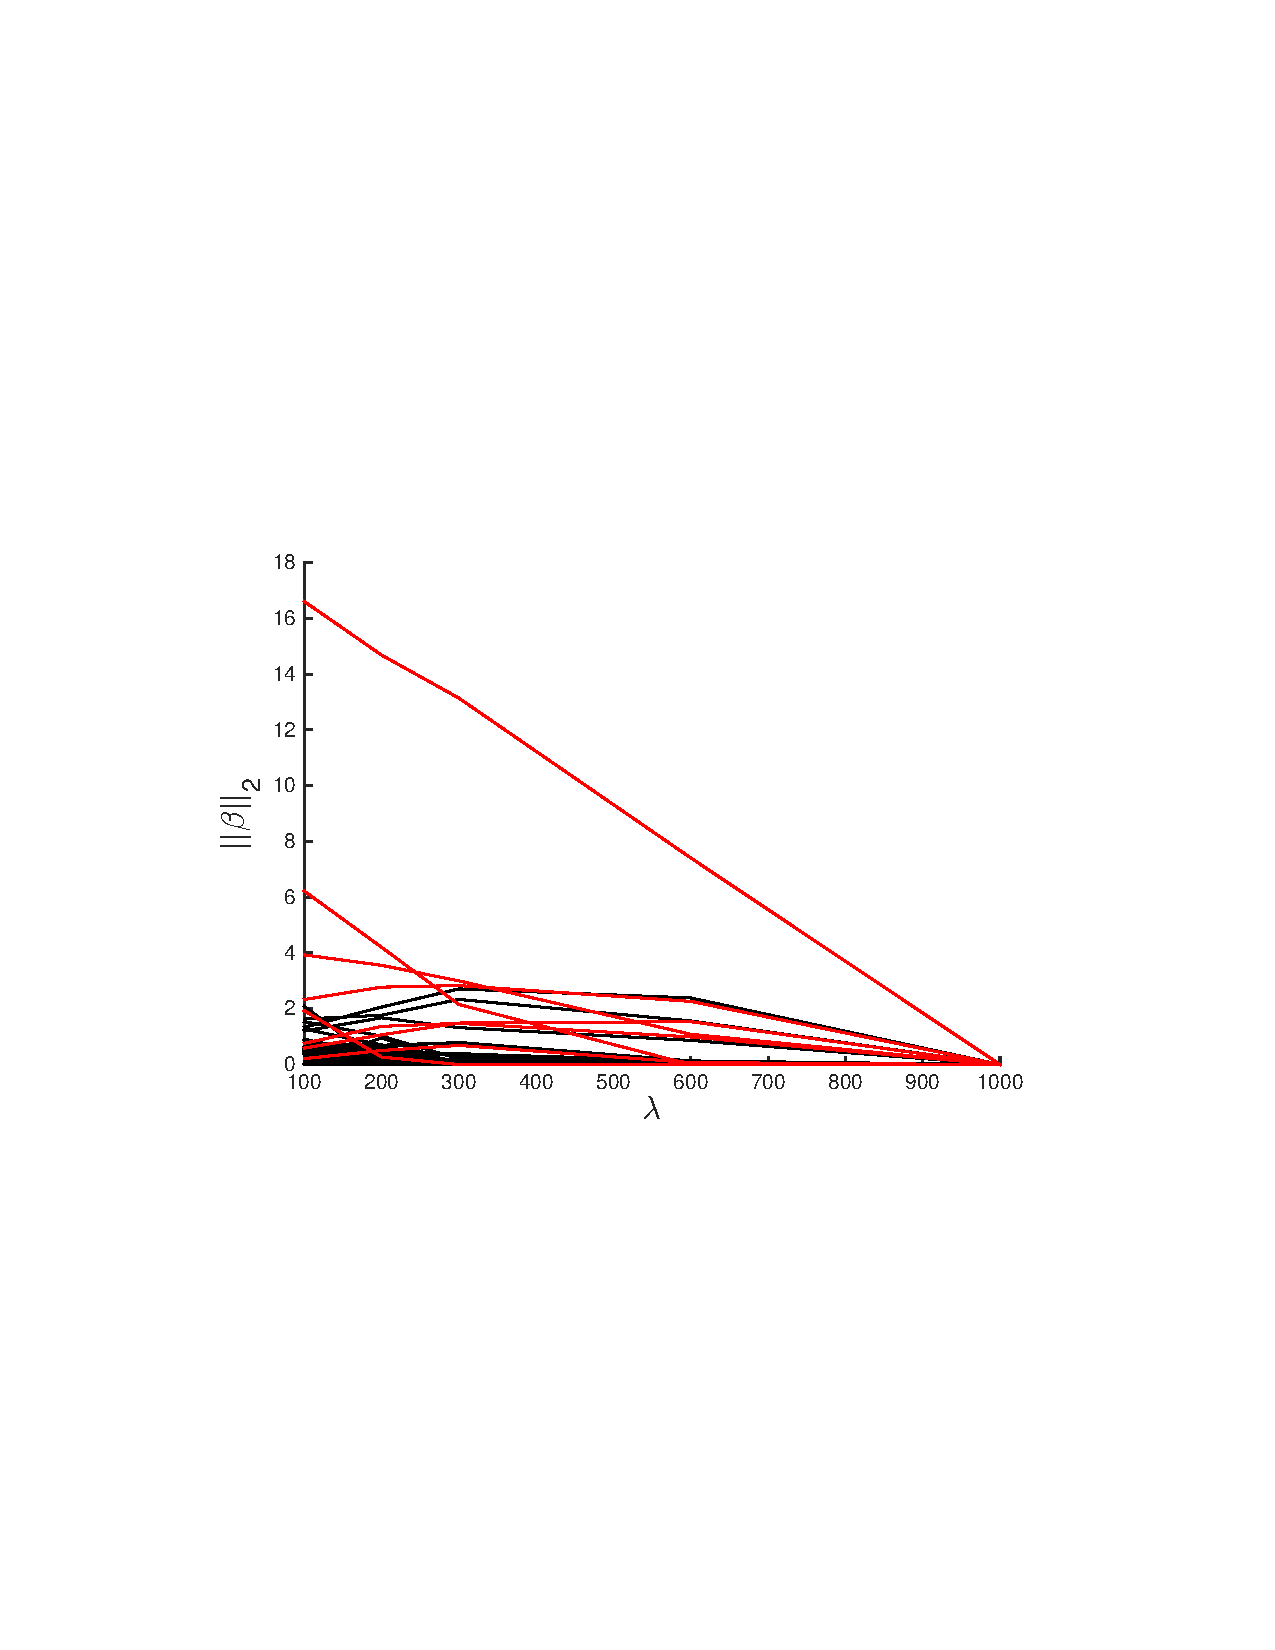
\includegraphics[width=3.2in]{figs/solnpath600.pdf}
\vspace{\imcaptionspace}
\caption[]{\small Solution path with $n=200$ samples (above) and
$n=600$ (below). The $x$-axis shows the regularization parameter,
while the $y$-axis plots $\|\funcj\|_{\Hcalkj} = \|\betaj\|$. 
The true nonzero functiosn are depicted in red. As the figure indicates, several
of the false functions are driven to $0$ fast whereas the true functions
persist for longer.
}
\vspace{\imtextspace}
\label{fig:n200}
\end{figure}
}


\newcommand{\insertTableRealData}{
\begin{table*}
\centering
\begin{tabular}{l|c|c|c|c|c|c|c|c}
Dataset ($D$, $n$) & \addkrr & \krr & \knn & \nw & \locallin & \localquad & \gp  & \svr \\
\hline \\[-0.16in]
\hline 
Speech ($21$, $520$) & $\bf{0.02269}$ & $0.02777$ & $0.09348$ 
  & $0.11207$ & $0.03373$ 
        & $0.02407$ & $0.02531$ & $0.22431$  \\
\hline
Music ($90$, $1000$) & $\bf{0.91627}$ & $0.91922$ & $1.00001$ 
      & $1.05745$ & $1.25805$ 
        & $1.06482$ & $0.94329$ & $1.07009$ \\
\hline
Tele-motor ($19$, $300$) & $\bf{0.06059}$ & $0.06488$ & 
  $0.13957$ & $0.20119$ 
  & $0.09455$ & $0.08774$ & $0.06678$ & $0.38038$ \\
\hline
Housing ($12$, $256$) & $\bf{0.31285}$ & $0.35947$ & $0.43619$ & $0.42087$ 
  & $\bf{0.31219}$ & $0.35061$ & $0.67566$ & $1.15272$ \\
\hline
Blog ($91$, $700$) & $\bf{1.43288}$ & $1.53227$ & $1.73545$ & $1.49305$ & $1.69234$ 
     & $1.71321$ & $1.64429$ & $1.66705$ \\
\hline
Forest Fires ($10$, $210$) & $0.30675$ & $0.32618$ & $0.40565$ & $0.37199$ 
   & $0.35462$ & $0.33881$ & $\bf{0.29038}$ & $0.70154$ \\
\hline
Propulsion ($15$, $400$) & $0.04167$ & $0.01396$ & $0.15760$ & $0.11237$ & $0.182345$ &
             $0.19212$ & $\bf{0.00355}$ & $0.74511$ \\
\hline
\end{tabular}
\caption{
The test set errors of all methods on 7 datasets from the UCI repository.
The dimensionality and number of training points is indicated with the dataset.
The best method(s) for each dataset are in bold font. \addkrr gives the best
results in most of the datasets and is within the top 3 in all of the datasets.
In the Forest Fires dataset it is only slightly worse than \gp. In the
Propulsion dataset, \gp seems to significantly outperform all other methods.
}
\label{tb:realData}
\end{table*}
}


\setboolean{istwocolumn}{true}

\begin{abstract}
We describe additive kernel ridge regression, a generalisation of the kernel
ridge method for nonparametric regression.
...
\end{abstract}


% % figures and tables
% 
\newcommand{\insertFigCompToy}{
\begin{figure}
\centering
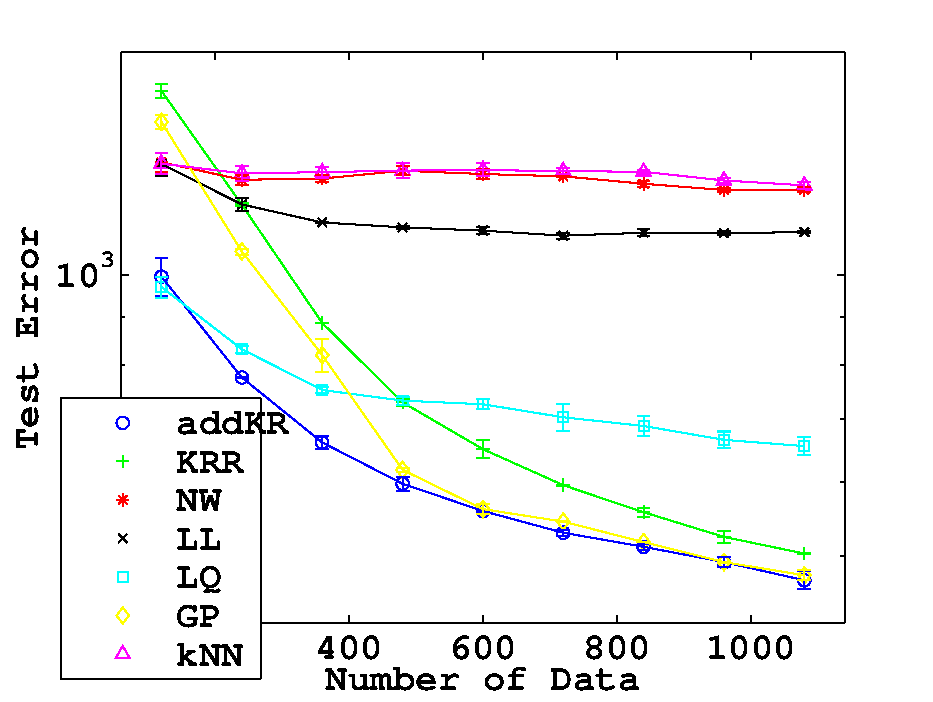
\includegraphics[width=3.2in]{figs/compToy}
\vspace{\imcaptionspace}
\caption[]{\small Comparison of various nonparametric regression methods on a
$20$-dimensional toy dataset. The $x$-axis denotes the number of training data
and the $y$-axis is the test error. }
\vspace{\imtextspace}
\label{fig:compToy}
\end{figure}
}

\newcommand{\insertFigOpt}{
\begin{figure}
\centering
\subfigure[]{
  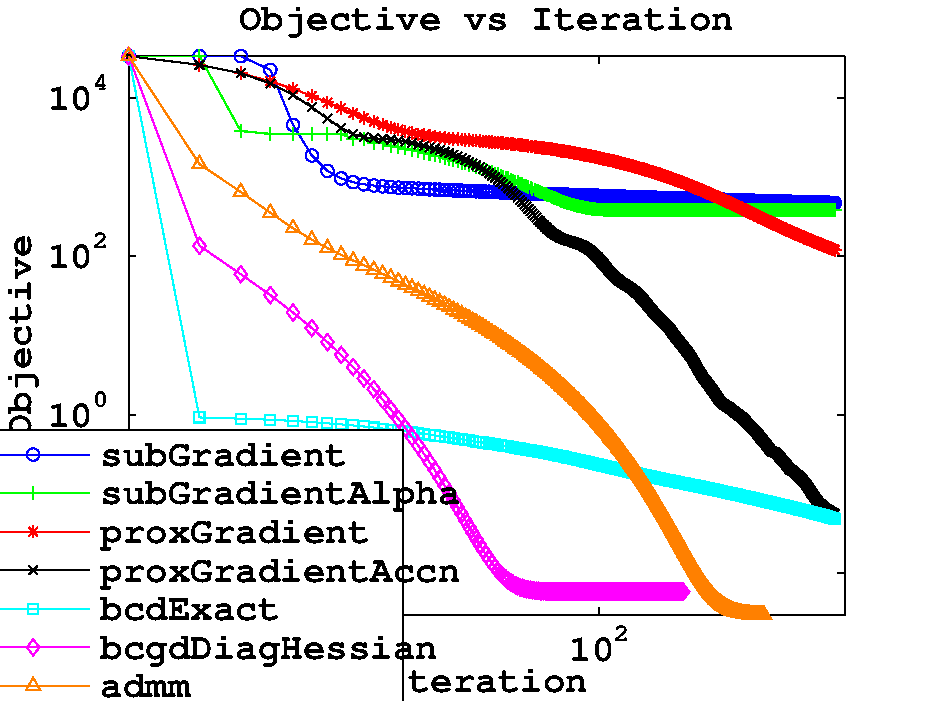
\includegraphics[width=\imarrwtwo]{figs/iteration1000v2} \hspace{\imhsptwo}
  \vspace{\imlabelspace}
  \label{fig:optCompIter}
}
\subfigure[]{
  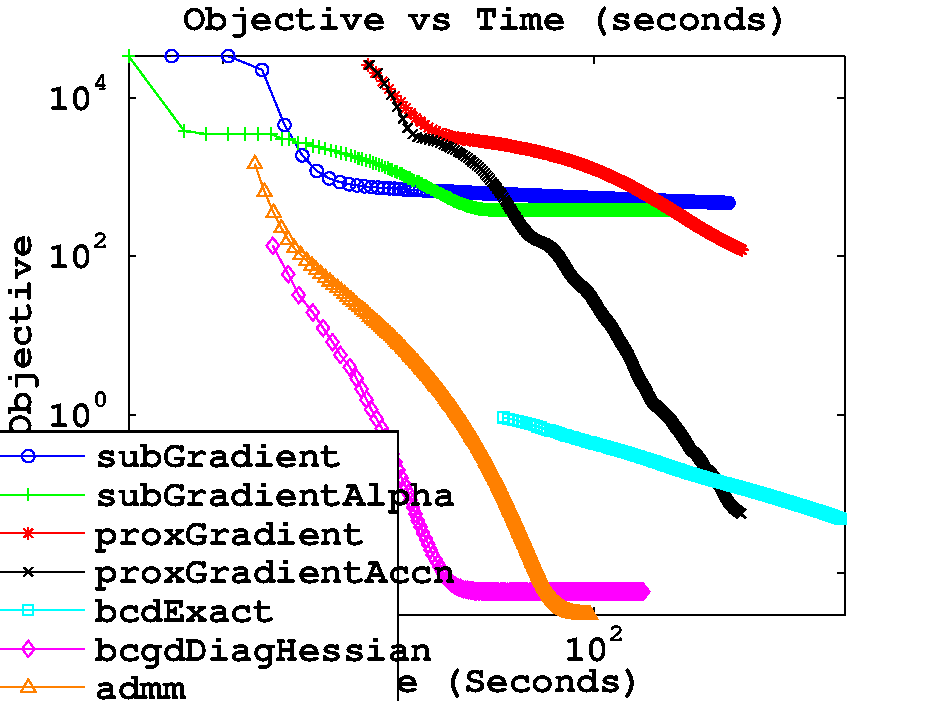
\includegraphics[width=\imarrwtwo]{figs/time1000v2} \hspace{\imhsptwo}
  \vspace{\imlabelspace}
  \label{fig:optCompTime}
}
\caption[]{\small
\subref{fig:optCompIter}: Comparison of the different methods to optimise our
objective. In~\subref{fig:optCompIter} The $x$-axis is the iteration and
in~\subref{fig:optCompTime} the $x$-axis is time. In both figures
 the $y$-axis is the objective. 
Both figures are in log-log scale.
}
\end{figure}
}

\newcommand{\insertFigRegFSel}{
\begin{figure}
\centering
\subfigure[]{
  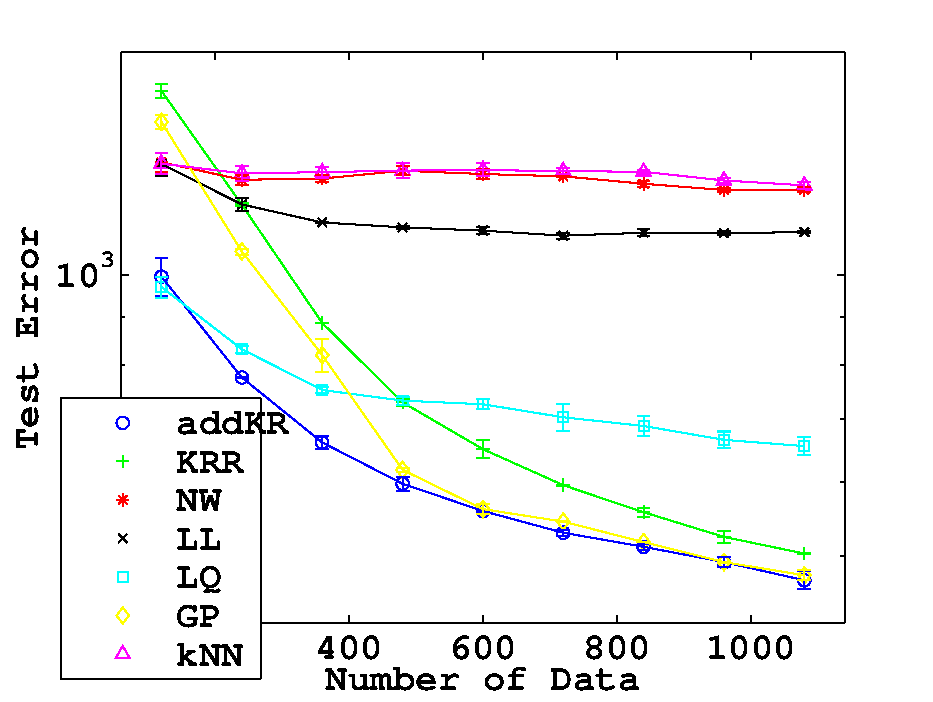
\includegraphics[width=\imarrwtwo]{figs/compToy} \hspace{\imhsptwo}
  \vspace{\imlabelspace}
  \label{fig:compToy}
}
\subfigure[]{
  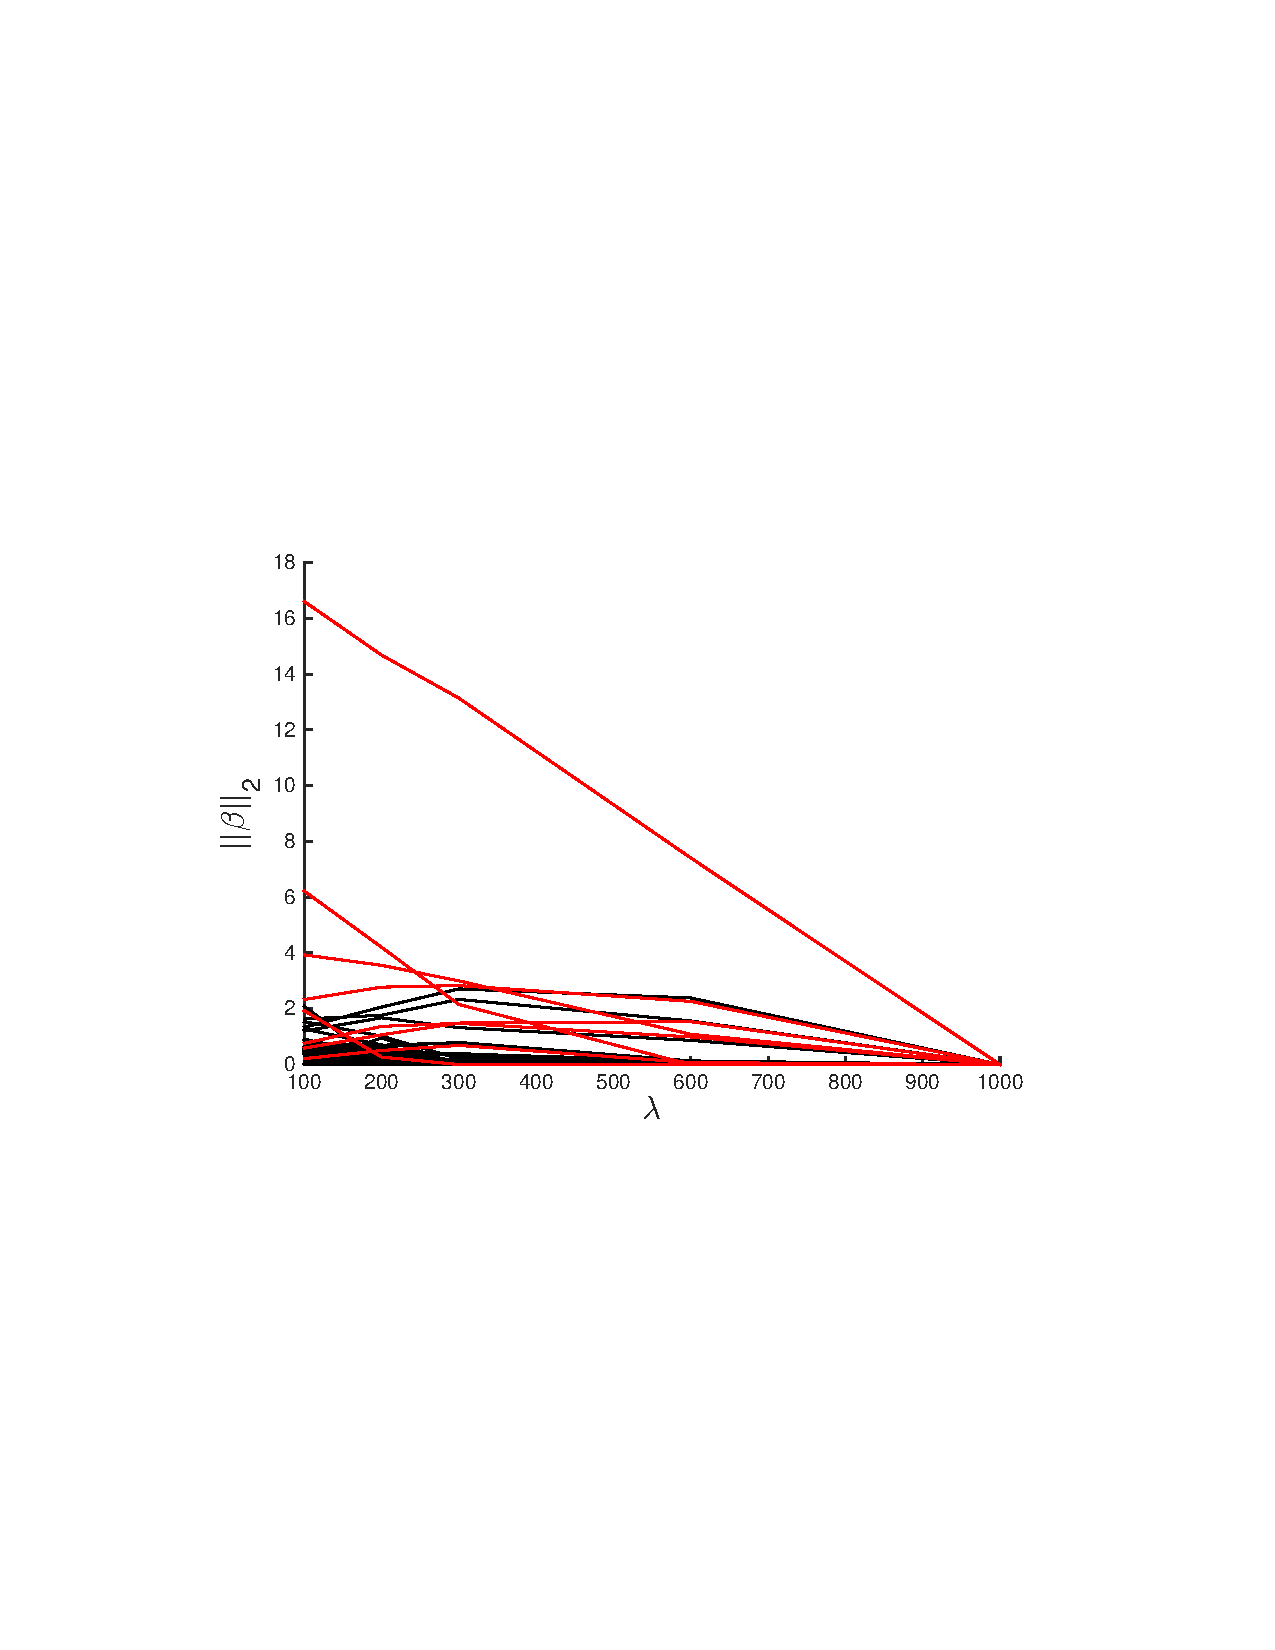
\includegraphics[width=\imarrwtwo]{figs/solnpath600} \hspace{\imhsptwo}
  \vspace{\imlabelspace}
  \label{fig:solnpath}
}
\caption[]{\small
\subref{fig:compToy}: Comparison of \addkrrs using ESP Kernels against other 
nonparametric methods
on a $20$ dimensional toy problem. The $x$-axis denotes the number of training
points and the $y$-axis is the error on a test set.
\subref{fig:solnpath}: Solution path with $n=600$ samples for the synthetic
problem. The $x$-axis shows the regularisation parameter while the $y$-axis
plots $\|\funcj\|_{\Hcalkj} = \|\betaj\|$. The true nonzero functions are
depicted in red. As the figure indicates several of the false functions are
driven to $0$ fast whereas the true functions persist for longer.
}
\end{figure}
}



\newcommand{\insertFigSolnPath}{
\begin{figure}
\centering
% 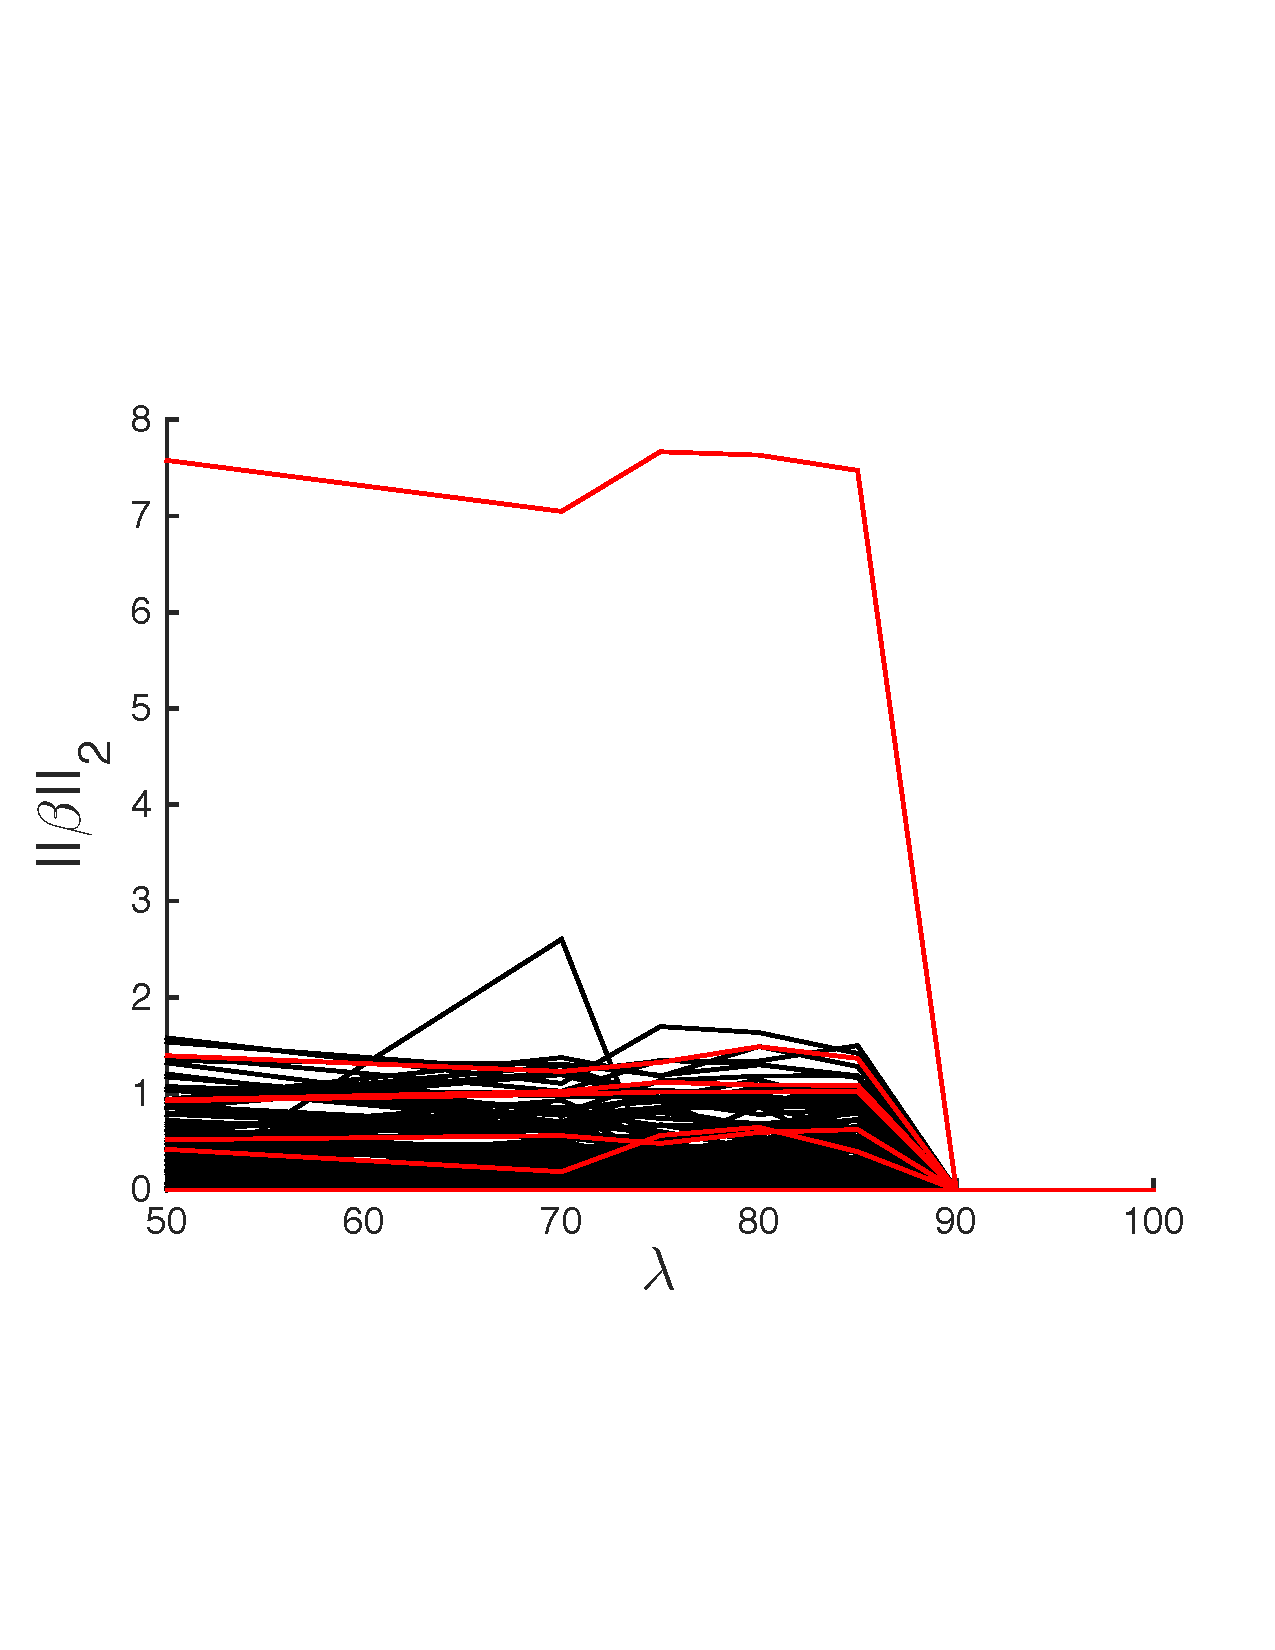
\includegraphics[width=3.4in]{figs/solnpath200.pdf}
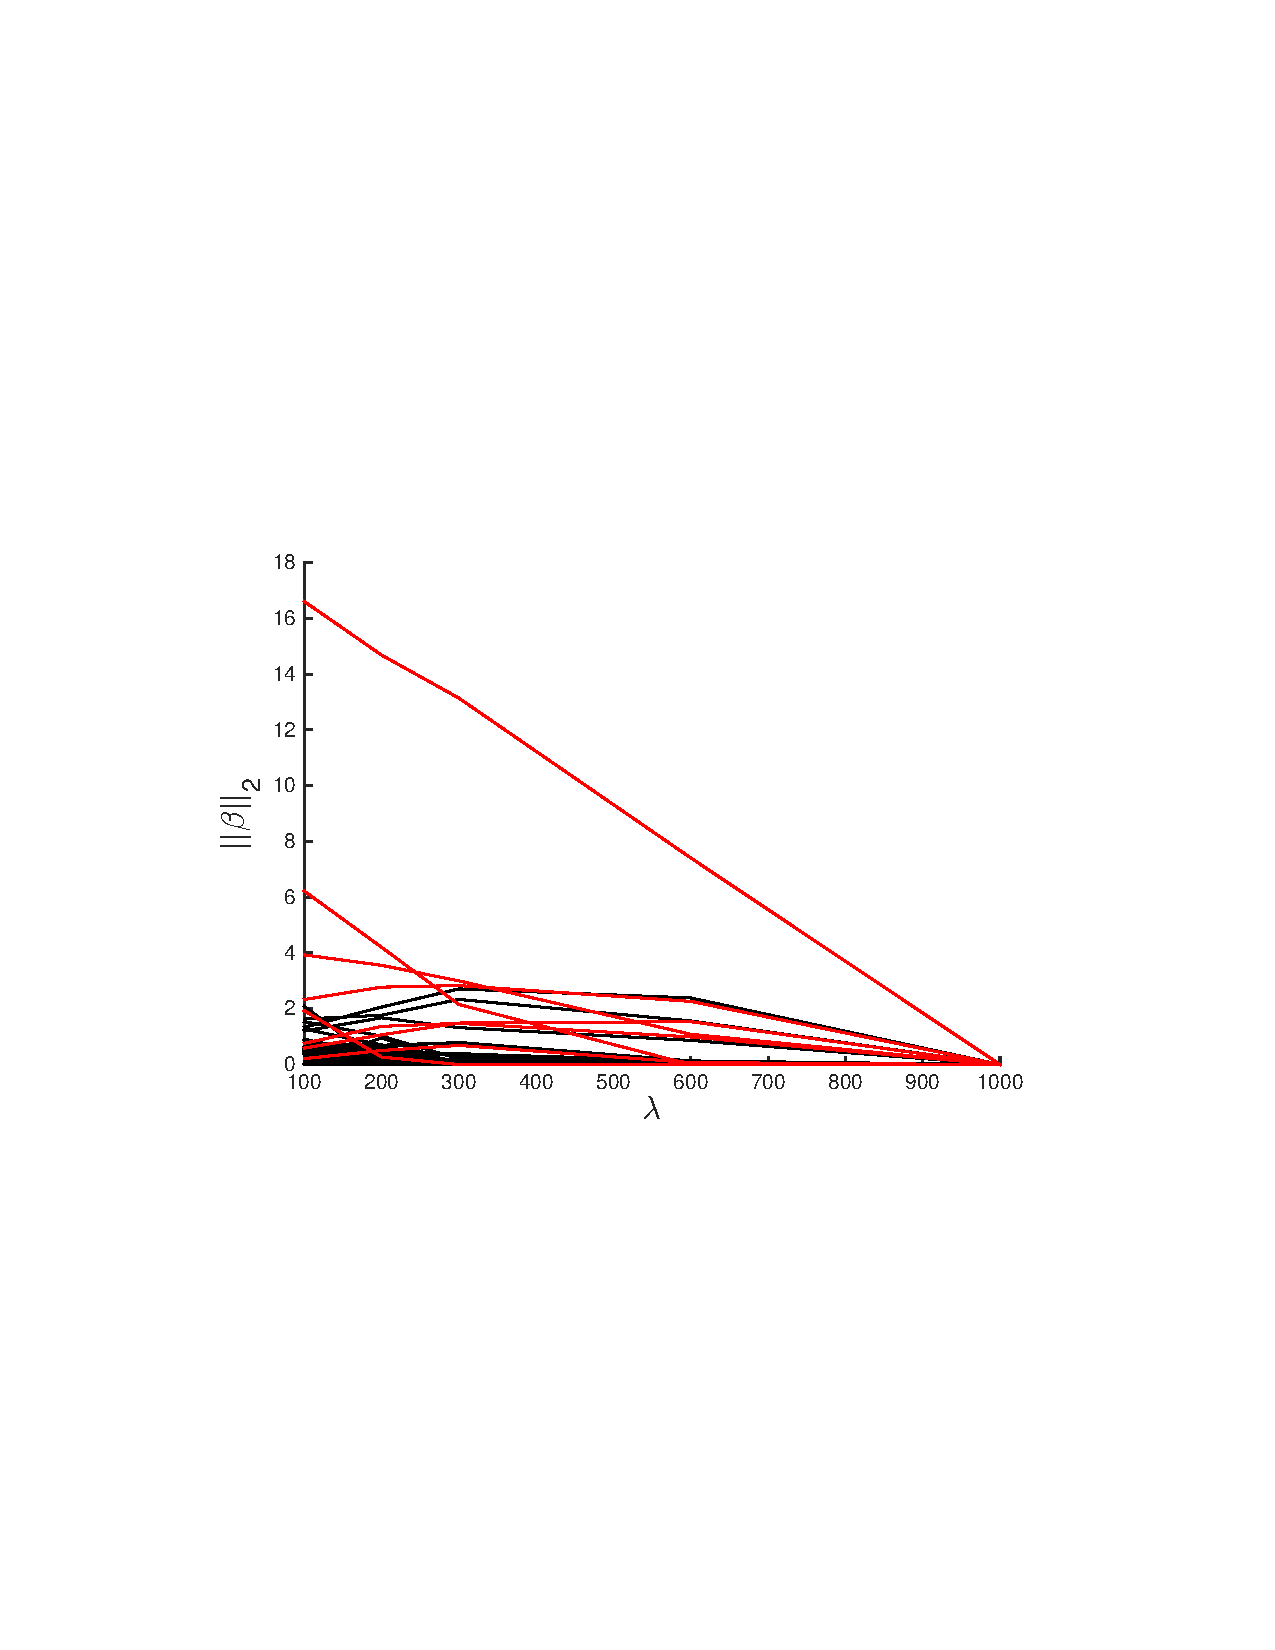
\includegraphics[width=3.2in]{figs/solnpath600.pdf}
\vspace{\imcaptionspace}
\caption[]{\small Solution path with $n=200$ samples (above) and
$n=600$ (below). The $x$-axis shows the regularization parameter,
while the $y$-axis plots $\|\funcj\|_{\Hcalkj} = \|\betaj\|$. 
The true nonzero functiosn are depicted in red. As the figure indicates, several
of the false functions are driven to $0$ fast whereas the true functions
persist for longer.
}
\vspace{\imtextspace}
\label{fig:n200}
\end{figure}
}

% 
\newcommand{\insertTableRealData}{
\begin{table*}
\centering
\begin{tabular}{l|c|c|c|c|c|c|c|c}
Dataset ($D$, $n$) & \addkrr & \krr & \knn & \nw & \locallin & \localquad & \gp  & \svr \\
\hline \\[-0.16in]
\hline 
Speech ($21$, $520$) & $\bf{0.02269}$ & $0.02777$ & $0.09348$ 
  & $0.11207$ & $0.03373$ 
        & $0.02407$ & $0.02531$ & $0.22431$  \\
\hline
Music ($90$, $1000$) & $\bf{0.91627}$ & $0.91922$ & $1.00001$ 
      & $1.05745$ & $1.25805$ 
        & $1.06482$ & $0.94329$ & $1.07009$ \\
\hline
Tele-motor ($19$, $300$) & $\bf{0.06059}$ & $0.06488$ & 
  $0.13957$ & $0.20119$ 
  & $0.09455$ & $0.08774$ & $0.06678$ & $0.38038$ \\
\hline
Housing ($12$, $256$) & $\bf{0.31285}$ & $0.35947$ & $0.43619$ & $0.42087$ 
  & $\bf{0.31219}$ & $0.35061$ & $0.67566$ & $1.15272$ \\
\hline
Blog ($91$, $700$) & $\bf{1.43288}$ & $1.53227$ & $1.73545$ & $1.49305$ & $1.69234$ 
     & $1.71321$ & $1.64429$ & $1.66705$ \\
\hline
Forest Fires ($10$, $210$) & $0.30675$ & $0.32618$ & $0.40565$ & $0.37199$ 
   & $0.35462$ & $0.33881$ & $\bf{0.29038}$ & $0.70154$ \\
\hline
Propulsion ($15$, $400$) & $0.04167$ & $0.01396$ & $0.15760$ & $0.11237$ & $0.182345$ &
             $0.19212$ & $\bf{0.00355}$ & $0.74511$ \\
\hline
\end{tabular}
\caption{
The test set errors of all methods on 7 datasets from the UCI repository.
The dimensionality and number of training points is indicated with the dataset.
The best method(s) for each dataset are in bold font. \addkrr gives the best
results in most of the datasets and is within the top 3 in all of the datasets.
In the Forest Fires dataset it is only slightly worse than \gp. In the
Propulsion dataset, \gp seems to significantly outperform all other methods.
}
\label{tb:realData}
\end{table*}
}




\section{Introduction}

Regression in high dimensions is an inherently difficult problem with known
lower bounds depending exponentially in dimension
\citep{gyorfi02distributionfree}. In this
project we intend to make progress in this problem by treating the function as
an additive model of lower dimensional components.
Using additive models is fairly standard in high dimensional regression
literature \cite{hastie90gam,ravikumar09spam,lafferty05rodeo}. 
However, we wish to consider additive models which are more expressive than
previous work.

We choose to model the low-order interaction basis functions implicitly using kernels.
We then minimize the squared-error loss combined with 
a squared RKHS norm penalty to enforce smoothness
and a mixed $\ell_{1,2}$-norm (group lasso style) penalty 
to limit the number of non-zero basis functions.
This leads to a convex objective function where the number of parameters is
the product of the number of samples and the number of basis functions.

Our work extends Sparse Additive Models (SpAM) \citep{ravikumar09spam} 
to multidimensional nonparametric basis functions.
Our proposed method also extends recent work on 
Generalized Additive Models plus Interactions \citep{intelligible:2013}.
However, in this work the interaction model was assumed to follow a specific functional form,
leading to an optimization method tailored to their interaction model.
Our research is also related to existing work on 
using linear combinations of kernels for kernel learning,
called multiple kernel learning \citep{mkl-review:2011}.

Optimization for our proposed method is complicated by 
the non-smooth $\ell_{1,2}$-norm regularization penalty.
Algorithms for group lasso have addressed this problem 
through a variety of approaches.
Proximal gradient \citep{beck2009fast}
has cheap iterations and relatively fast convergence if combined with acceleration.
An block coordinate descent method has also been developed \citep{bcd-group-lasso:2013}.
Further, the general Coordinate Gradient Descent method \citep{cgd:2009} 
can also be specialized to $\ell_{1,2}$-penalized problems 
\citep{meier2008group,note-group-lasso:2010}.
Recent work \citep{group-fused-lasso:2014} on the group fused lasso 
has sidestepped the $\ell_{1,2}$-norm penalty, transforming it to a 
smooth objective with non-negativity constraint.
Finally, safe screening rules for the group lasso have been developed 
\citep{group-lasso-screening:2013} which quickly eliminate many of the all-0 
groups.

For Sparse Additive Models, parameters are typically 
optimized via the backfitting algorithm \citep{ravikumar09spam}, 
a special case of (block) coordinate descent with group sizes of 1.



\section{Problem Set up \& Algorithm}
\label{sec:additiveKR}

\subsection{Problem Statement \& Notation}
\label{sec:setup}

Let $\func : \Xcal \rightarrow \RR$ be the function of interest. 
Here $\Xcal \ni x = [x_1, \dots, x_D] \in \RR^D$ and $\Xcal \subset \RR^D$.
We have data $\XYn$ and wish to obtain an estimate
$\funchat$ of $\func$.
In this work, we seek an additive approximation to the
function. That is, $\funchat$ can be expressed as,
\begin{align*}
\funchat(x) = \funchatii{1}(x) + \funchatii{2}(x) + \dots +
\funchatii{M}(x)
\numberthis
\label{eqn:addAssumption}
\end{align*}
where each $\funchatii{j}:\Xcal \rightarrow \RR$.
% where $\xii{j} \in \Xcalj \subset \RR^{d_j}$ and $\funchatj:\Xcalj \rightarrow
% \RR$. We shall refer to the $\Xcalj$'s as \emph{groups} and the collection of all
% groups $\bigcup_{j=1}^M \Xcalj$ as the \emph{decomposition}.
% We are particularly  interested in the case
% where $D$ is very large and the group dimensionality is bounded-- i.e. $d_j \leq
% d \ll D$. 

The work in \citet{hastie90gam} treats $\funchat$ as a sum of one
dimensional components. 
In Equation~\eqref{eqn:addAssumption}
this corresponds to setting $M=D$ and have each $\funchatii{j}$ act on only the
$j$\superscript{th} coordinate.
% The decomposition here corresponds to
% $\xii{j} = x_j$, $d_j = d =1\; \forall j$ and $M = D$. 
In this work, we would like to be more expressive than this model. We will
consider additive models on more than just one dimension and more importantly allows for
overlap between the groups. For e.g. $\funchat(x_1, x_2,
x_3) = \funchatii{1}(x_1) + \funchatii{2}(x_1, x_2) + \funchatii{3}(x_2, x_3)$.
\citet{ravikumar09spam} treat $\funchat$ as a sparse combination of one
dimensional functions. While this is seemingly restrictive than
\citep{hastie90gam}, the sparse approximation may provide favourable
bias-variance tradeoffs in high dimensions. Drawing inspiration from this, we
will also consider models where $M$ is very large and seek a sparse collection of
groups to approximate the function - i.e. $\funchatj = \zero$ for several $j$.


\subsection{Additive Least Squares Regression via Kernels}
\label{sec:addKR}

One of several ways to formulate a nonparametric regression problem is to 
minimise an
objective of the form $J(f) = \sum_{i=1}^n \ell(f(X_i), Y_i) + \lambda P(f)$ 
over a nonparametric class of functions $\Fcal$.
Here $\ell$ is a loss function and $P$ is a term that penalises the complexity
of the function $f$. Several nonparametric regression problems such as Gaussian
processes, smoothing splines and natural splines can be formulated this way.
Or particular interest to us is Kernel Ridge Regression (\krr)
which uses a positive semidefinite kernel 
$\kernel: \Xcal \times \Xcal \rightarrow \RR$ \citep{scholkopf01kernels}
and takes $\Fcal$ is taken to be the reproducing kernel Hilbert
space (RKHS) $\Hcal_\kernel$ corresponding to $\kernel$. $P$ is taken to be 
the squared RKHS norm of $f$ and $\ell$ the squared error loss. 
Accordingly, \krrs is characterised via the optimisation objective,
\[
\funchat = \argmin_{f \in \Hcal_\kernel} \sum_{i=1}^n (Y_i - f(X_i))^2 +
\lambda \|f\|^2_\Hcalk
\]
However, like most nonparametric regression models, \krrs suffers from the curse of
dimensionality. To obtain an additive approximation we consider $M$ kernels
$\kernelj$ and their associated RKHSs $\Hcalkj$. In
equation~\eqref{eqn:addAssumption}, we will aim for $\funchatj \in \Hcalkj$.
Accordinly we consider an optimisation problem of the following form where
we jointly optimise over $\funchatii{1}, \dots, \funchatii{M}$,
\begin{align*}
& \{\funchatj\}_{j=1}^M =
\argmin_{\funcj \in \Hcalkj, j = 1,\dots, M} 
  F\left( \{\funcj\}_{j=1}^M \right) \\
& \textrm{where, } 
  \numberthis \label{eqn:rkhsObjective}
\\
& F\left( \{\funcj\}_{j=1}^M \right)  \;=  \\
&\hspace{0.2in}  
  \frac{1}{2}\sum_{i=1}^n \left(Y_i - \sum_{j=1}^M \funcj (\xj) \right)^2 
 + \lambda \sum_{j=1}^M \|\funcj\|^q_\Hcalkj 
\end{align*}
Our estimate for $\func$ is then $\funchat(\cdot) = \sum_j \funchatj(\cdot)$.

Via a representer theorem like argument it is straightforward to show
that $\funcj$ will be in the linear span of the reprodcing kernel maps of the
training points $\Xn$ -- i.e. $\funcj(\cdot) = 
\sum_j \alphaj_i \kernelj(\cdot, X_i) $.
Then, the $j$\superscript{th} term in the second summation can be written as
${\alphaj}^\top \KKj \alphaj$,
where $\KKj \in \RR^{n\times n}\; \forall
j$ such that $\KKj_{rc} = \kernelj(X_r, X_c)$.
After further simplification, the objective can be written as,
$\aalpha = \argmin_{\aalpha \in \RR^{nM}} F(\aalpha)$ where,
\begin{equation}
\Falpha(\aalpha) = \frac{1}{2}\Big\|Y - \sum_{j=1}^m \KKj \alphaj\Big\|_2^2 + 
  \lambda \sum_{j=1}^M \left({\alphaj}^\top \KKj \alphaj\right)^{q/2}.
%   \lambda \sum_{j=1}^M \sqrt{{\alphaj}^\top \KKj \alphaj}^{q/2}.
\label{eqn:optObjective}
\end{equation}
Here $\alphaj \in \RR^n \; \forall j$, $\aalpha = [{\alphaii{1}}^\top, \dots, 
{\alphaii{M}}^\top]^\top  \in\RR^{nM}$ and $Y = [Y_1, \dots, Y_n]^\top \in
\RR^n$. Given the solution to the above, our
estimate is obtained via $\funchat(\cdot) = \sum_{j=1}^M \sum_{i=1}^n \alphaj_i
\kernelj(\cdot, \Xj_i)$.
Equation~\eqref{eqn:optObjective} will the (convex) optimisation problem in our
algorithm.
We call this algorithm Additive Kernel Regression (\addkrr).
A natural choice for $q$ in the objective~\eqref{eqn:rkhsObjective} is $q=2$. 
However in
this work we use $q=1$ since it encourages a sparse subset of functions as the
solution which provides interpretability of the learned models. 


\subsection{Choice of Kernels}

All that is left to do to complete the specification of our algorithm is to
describe the construction of the kernels $\kernelj$. We consider two settings
in this regard.

The first is when we wish to reduce the statistical complexity of the function
we to be learned in high dimension. A kernel directly defined on $D$ dimensions
is complex since it allows for interactions of all $D$ variables. We may reduce
the complexity of the kernel by constraining how these variables interact.
In particular we consider kernels of the form, 
\begin{align*}
\kernelii{1}(x,x') &= \sum_{1\leq i \leq D} \kerni(x_i, x'_i) 
\numberthis \label{eqn:espKernel} \\
\kernelii{2}(x,x') &= \sum_{1\leq i_1 < i_2 \leq D} 
\kernel_{i_1}(x_{i_1},x'_{i_1})  \kernel_{i_2}(x_{i_2},x'_{i_2})\\
\kernelii{M}(x,x') &= \sum_{1\leq i_1 < i_2 < \dots < i_M \leq D} 
  \prod_{d=1}^M \kernel_{i_d}(x_{i_d}, x'_{i_d}) 
\end{align*}
Here $\kerni:\RR\times\RR \rightarrow \RR$ 
is a base kernel acting on one dimension. 
$\kernelj$ has ${D \choose j}$ terms and exhaustively computing all of them is
computationally intractable.
Fortunately, by observing that the $j$\superscript{th} kernel is just the
$j$\superscript{th} elementary symmetric polynomial (ESP) on the base kernel values we
may use the Newton Girard formula to efficiently compute them recursively.
Precisely, by denoting $\kappa_s = \sum_{i=1}^D (\kernel_i(x_i, x'_i))^s$ 
we have, 
\[
\kernelii{j}(x,x') = \frac{1}{j} \sum_{d=1}^j (-1)^{d-1} 
  \;\kappa_j \; \kernelii{j-d}(x, x')
\]
Computing the $M$ kernels this way only requires $O(DM)$ computation.
We call this choice of kernels the \emph{ESP Kernels}.
A similar kernel using a similar trick for computing it was used in
\citet{duvenaud11additivegps}.

% \textbf{Setting 2 (Function Selection): }
The second setting is when we are explicitly searching for a sparse subset of
functions to explain the data. For instance, in neurological models, while the
function of interest has several variables the interactions are sparse and of
lower order. For example, a function of $4$ variables may take the form
\[
f(x) = \funcii{1}(x_1) + \funcii{2}(x_2,x_3) + \funcii{3}(x_1, x_4)
\]
That is, the function decomposes as a sum of functions acting on small groups of
variables. Given a large set of candidate groups, the task at hand is to
recover the groups and the individual functions acting on those groups.
In this setting, $M$ and our RKHSs are determined by the problem
-- $\Hcalkj$ contains functions on the variables
belonging to the $j$\superscript{th} candidate group. 


\subsection{Implementation}

We now describe the implementation and other detials of the above algorithm.
Let the Cholesky decomposition of $\KKj$ be $\KKj = \LLj \LLj^\top$. 
Denote $\betaj = \LLj^\top \alphaj$.
Then, our objective can be written in terms of $\bbeta = [{\betaii{1}}^\top,
\dots, {\betaii{M}}^\top]$ as,
\begin{equation}
\Fbeta(\bbeta) =  \frac{1}{2}\Big\|Y - \sum_{j=1}^m \LLj \alphaj\Big\|_2^2 + 
  \lambda \sum_{j=1}^M \|\betaj\|_2
\end{equation}
The objective, in the above form is well studied in optimisation literature as the group
LASSO. 
When the number of parameters for each group are small, which is
typically the case in group LASSO problems, block coordinate descent (BCD) is believed
to be the state of the art solver. However, in our case the number of parameters
is large -- growing linearly with $n$. In this regime BCD is slow since it
requires a matrix inversion at each step. In particular, we found that Block
Coordinate Gradient Descent (BCGD) significantly outperformed BCD in our
experiments. 
In fact, we tried several other methods including subgradient method, proximal
gradient method and ADMM and found that BCGD performed best.

The penalty term $\lambda$ was chosen using $5$-fold cross validation. Our implementation
first solves for the largest $\lambda$ value. For successive $\lambda$
values, we initialise BCGD at the solution of the previous $\lambda$ value. This
warm starts procedure significantly speeds up the running time of the entire
training procedure.


\section{Experiments}
\label{sec:experiments}

\insertTableRealData

\subsection{Setting 1: ESP Kernels for High Dimensional Regression}

In our implementations of the ESP kernels, for the one dimensional base kernel we use
the RBF kernel $\kerni(x,x') = \exp((x-x')^2/h^2)$ with bandwidth $h$.
Since cross validating on all the kernel bandwidths is expensive, we set
it to $h = c\sigma n^{-0.2}$. This follows other literature 
\cite{gyorfi02distributionfree,ravikumar09spam} using similar choices for kernel
bandwidths. The constant $c$ was hand tuned -- we found that the performance of
our methods was robust to choices of $c$ between $5$ and $40$.
The value of $M$ was also hand tuned and set to $M = \min(D/4, 10)$.

We compare \addkrrs against kernel kidge regression(\krr),
Nadaraya Watson regression (\nw), locally linear regression (\locallin), locally
quadratic regression (\localquad), Gaussian process regression (\gp), $k$
nearest neighbors regression (\knn) and support vector regression (\svr).
For \gps and \svrs we use the implementations in
\citet{rasmussen10gpml,chang11libsvm} respectively.
For the other methods, we chose hyper parameters using $5$-fold cross
validation.
The Additive Gaussian process model of \citet{duvenaud11additivegps} is also a
candidate but we found that inference was extremely slow beyond a few hundred
training points (For e.g. it took $> 50$ minutes with $600$ points whereas
\addkrrs ran in under $4$ minutes).

First, we construct a smooth synthetic 20 dimensional function. We train all methods on
$n$ training points where $n$ varies from $100$ to $1100$ and test on $1000$
points sampled independently. The results are shown in Figure~\ref{fig:compToy}.
\addkrrs outperforms all other methods. We suspect that \nw, \locallins and \knns perform
very poorly since they make very weak smoothness assumptions about the function.

Next, we compare all methods on $7$ moderate to high dimensional datasets from the UCI
repository. All inputs and labels were preprocessed to have zero mean and unit
standard deviation. We split the datasets into roughly two halves for training
and testing. The results are given in Table~\ref{tb:realData}. Our proposed
method outperforms alternatives in most cases.

\insertFigRegFSel

% 
\subsection{Setting 2: Function Selection}

In this work, we use RBF kernels on each group by setting kernel bandwidths
for each dimension as same as above.


\subsection{Setting 2: Function Selection}

In this section, we study the ability of our method to recover the true function.
We use RBF kernels on each group by setting kernel bandwidths
for each dimension as same as explained above.
% Extending the generative model in \cite{ravikumar09spam}, 

First, we conduct the following synthetic experiment.
We generate $600$ observations from the following
50-dimensional additive model:
\begingroup
\allowdisplaybreaks
\begin{align*}
	y_i =& f_1(x_{i1}) + f_2(x_{i2}) + f_3(x_{i3}) + f_4(x_{i4}) + 
f_1(x_{i5}x_{i6}) + f_2(x_{i7}x_{i8}) + 
f_3(x_{i9}x_{i10}) + f_4(x_{i11}x_{i12}) + \epsilon_i 
\end{align*}
\endgroup
where,
\begin{align*}
f_1(x) = -2\sin(2x), \;\; f_2(x) = x^2 - \frac{1}{3}, \;\;
f_3(x)= x-\frac{1}{2}, f_4(x) = e^{-x} + e^{-1} - 1
\end{align*}
% \begingroup
% \allowdisplaybreaks
% \begin{align*}
% 	y_i =& f_1(x_{i1}) + f_2(x_{i2}) + f_3(x_{i3}) + f_4(x_{i4}) + \\
% &f_1(x_{i5}x_{i6}) + f_2(x_{i7}x_{i8}) + \\
% &f_3(x_{i9}x_{i10}) + f_4(x_{i11}x_{i12}) + \epsilon_i \\
% f_1(x) =& -2\sin(2x), f_2(x) = x^2 - \frac{1}{3}, \\
% f_3(x)=& x-\frac{1}{2}, f_4(x) = e^{-x} + e^{-1} - 1
% \end{align*}
% \endgroup
with noise $\epsilon_i \sim \mathcal{N}(0,1)$.
Thus, 46 out of 50 individual features are irrelevant, and
1221 out of 1225 pairwise features are irrelevant.
As candidates, we use all functions of first and second order interactions --
i.e the kernels charactersing our RKHSs are of the form
$k(x_i, x'_i)$ for $i=1,\dots,50$ and $k(x_i,x_i)k(x_j,x_j)$ for
$1\leq i < j \leq 50$. Therefore, in this experiment $M = 1275$.

We plot the solution path for two independent datasets. The plots give the RKHS
norm of the function on each kernel $\|\funchatj\|_{\Hcalkj} = \|\betaj\|_2$
for all kernels against the value of the regularization parameter $\lambda$.
The results are shown in Figure~\ref{fig:solnpath}. 
At $\lambda=200$ we recover all true nonzero functions for a true positive rate
of $100\%$ and have 47 false negatives for a false positive rate of $3.7\%$




% Bibliography 
\bibliography{kky,convexopt}
\bibliographystyle{icml2015}

\end{document} 


% This document was modified from the file originally made available by
% Pat Langley and Andrea Danyluk for ICML-2K. This version was
% created by Lise Getoor and Tobias Scheffer, it was slightly modified  
% from the 2010 version by Thorsten Joachims & Johannes Fuernkranz, 
% slightly modified from the 2009 version by Kiri Wagstaff and 
% Sam Roweis's 2008 version, which is slightly modified from 
% Prasad Tadepalli's 2007 version which is a lightly 
% changed version of the previous year's version by Andrew Moore, 
% which was in turn edited from those of Kristian Kersting and 
% Codrina Lauth. Alex Smola contributed to the algorithmic style files.  
